\subsection{Scopo del progetto}

Lo scopo del progetto è quello di implementare un modulo hardware, descritto in VHDL, che applichi il codice convoluzionale $\frac{1}{2}$ ad un flusso di bit salvato in memoria. Il flusso di bit generato dovrà essere a sua volta memorizzato.

\subsection{Codice convoluzionale \texorpdfstring{$\frac{1}{2}$}{}}
\label{section:convolutore}

Un codice convoluzionale è un tipo di codifica nel quale l'informazione, composta da \textit{m} bit, viene trasformata in un flusso di \textit{n} bit, dove \textit{m/n} è il rapporto del codice o tasso di trasmissione.\footcite{codiceconvoluzionale}

Nel caso in esame, il codice convoluzionale ha un rapporto $\frac{1}{2}$, quindi per ogni bit di informazione vengono generati due bit. Per il calcolo del flusso in uscita viene seguito lo schema riportato in figura \ref{fig:codificatore} dove i nodi rettangolari rappresentano dei flip flop e i nodi rotondi delle somme.

\tikzstyle{addnode} = [circle, draw=gray!60, fill=gray!5, very thick, minimum size=7.5mm]
\tikzstyle{flipflop} = [rectangle, draw=gray!60, fill=gray!5, very thick, minimum width=20mm, minimum height=10mm]

\begin{figure}[!ht]
    \centering
    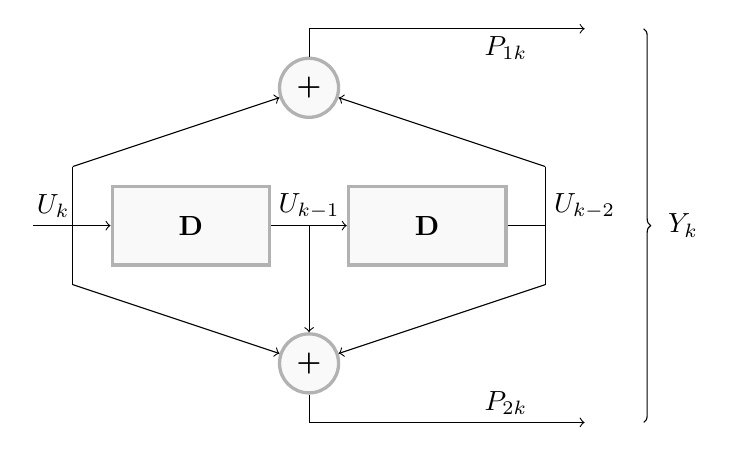
\begin{tikzpicture}[node distance=4cm]
        \node(ff1)  at (0, 0) [flipflop] {\textbf{D}};
        \node(ff2)  at (3, 0) [flipflop] {\textbf{D}};
        \node(add1) at (1.5, 1.75) [addnode] {\textbf{+}};
        \node(add2) at (1.5, -1.75) [addnode] {\textbf{+}};

        \draw[->] (-2, 0) -- (ff1.west);
        \draw[->] (ff1.east) -- (ff2.west);
        \draw[-] (ff2.east) -- (4.5, 0);

        \draw[-] (-1.5, 0) -- (-1.5, 0.75);
        \draw[->] (-1.5, 0.75) -- (add1);
        \draw[-] (4.5, 0) -- (4.5, 0.75);
        \draw[->] (4.5, 0.75) -- (add1);

        \draw[-] (-1.5, 0) -- (-1.5, -0.75);
        \draw[->] (-1.5, -0.75) -- (add2);
        \draw[-] (1.5, 0) -- (1.5, -0.75);
        \draw[->] (1.5, -0.75) -- (add2);
        \draw[-] (4.5, 0) -- (4.5, -0.75);
        \draw[->] (4.5, -0.75) -- (add2);

        \draw[-] (add1) -- (1.5, 2.5);
        \draw[->] (1.5, 2.5) -- (5, 2.5);
        \draw[-] (add2) -- (1.5, -2.5);
        \draw[->] (1.5, -2.5) -- (5, -2.5);

        \draw [decorate, decoration = {brace}] (5.75, 2.5) -- (5.75, -2.5);

        \node at (-1.75, 0.25) {$U_k$};
        \node at (1.5, 0.25) {$U_{k-1}$};
        \node at (5, 0.25) {$U_{k-2}$};
        \node at (4, 2.25) {$P_{1k}$};
        \node at (4, -2.25) {$P_{2k}$};
        \node at (6.25, 0) {$Y_k$};
    \end{tikzpicture}
    \caption{Codificatore convoluzionale con tasso di trasmissione $\frac{1}{2}$}
    \label{fig:codificatore}
\end{figure}

Considerando il flusso $U$ di bit in ingresso e indicando con $k$ l'instante di tempo considerato, la codifica legge il bit $U_k$ e produce i bit $P_{1k}$ e $P_{2k}$ calcolati come mostrato in eq. \ref{eq:p1k} e \ref{eq:p2k}. È importate sottolineare che il convolutore mantiene in memoria, ad ogni istante di tempo, gli ultimi due bit precedentemente letti, ovvero $U_{k-1}$ e $U_{k-2}$, i quali sono inizializzati a $0$. Inoltre, per produrre i bit di $P$, viene applicato l'operatore XOR ($\oplus$) in modo tale da ottenere una somma senza riporto.

\begin{equation}
    P_{1k} = U_k \oplus U_{k-2}
    \label{eq:p1k}
\end{equation}
\begin{equation}
    P_{2k} = U_k \oplus U_{k-1} \oplus U_{k-2}
    \label{eq:p2k}
\end{equation}

Il flusso in uscita sarà la concatenazione dei bit $P_{1k}$ e $P_{2k}$. Il convolutore è quindi una macchina sequenziale sincrona con un clock globale che scandisce l'ingresso dei bit del flusso $U$ e il calcolo dei bit di $P$.

\newpage

In figura \ref{table:esempio8bit} è riportato un esempio in cui vengono codificati 8 bit. Il flusso in uscita è quindi composto come: $P_{10},P_{20},P_{11},P_{21},...,P_{17},P_{27}$.

\begin{figure}[!ht]
    \centering
    \begin{minipage}{0.4\linewidth}
        \begin{tabular}{c | c | c | c | c | c | c | c | c}
            T        & 0 & 1 & 2 & 3 & 4 & 5 & 6 & 7 \\
            \hline
            $U_k$    & 1 & 0 & 1 & 0 & 0 & 0 & 1 & 0 \\
            $P_{1k}$ & 1 & 0 & 0 & 0 & 1 & 0 & 1 & 0 \\
            $P_{2k}$ & 1 & 1 & 0 & 1 & 1 & 0 & 1 & 1 \\
        \end{tabular}
    \end{minipage}
    \begin{minipage}{0.4\linewidth}
        \begin{equation*}
            U = 10100010
        \end{equation*}
        \begin{equation*}
            P = 1101000111001101
        \end{equation*}
    \end{minipage}
    \caption{Esempio di codifica di 8 bit}
    \label{table:esempio8bit}
\end{figure}

\subsection{Descrizione della memoria}

Il modulo da implementare deve leggere il flusso $U$ da una memoria con indirizzamento al byte. All'indirizzo $0$ è presente la quantità di parole $W$ da codificare e, a partire dall'indirizzo $1$, i byte $U_k$. La dimensione massima della sequenza di ingesso è di $255$ byte. Il flusso in uscita dovrà essere memorizzato a partire dall'indirizzo $1000$.

In figura \ref{table:memoria} è rappresentato il contenuto della memoria.

\begin{figure}[!ht]
    \centering
    \begin{tabular}{c | c}
        Indirizzo   & Contenuto  \\
        \hline
        $0$         & $W$        \\
        $1$         & $U_0$      \\
        $2$         & $U_1$      \\
        ...         & ...        \\
        $W$         & $U_{W-1}$  \\
        ...         & ...        \\
        $1000$      & $P_{0}$    \\
        $1001$      & $P_{1}$    \\
        ...         & ...        \\
        $1000+2W-1$ & $P_{2W-1}$ \\
    \end{tabular}
    \caption{Contenuto della memoria}
    \label{table:memoria}
\end{figure}

\subsection{Specifiche di funzionamento}

Il componente da descrivere in VHDL deve implementare l'interfaccia indicata in figura \ref{code:interfacciacomponente} e rispettare le seguenti caratteristiche:

\begin{itemize}
    \item L'elaborazione parte quando il segnale \verb|i_start| viene portato a $1$;
    \item Il segnale \verb|o_done| deve essere portato a $1$ per indicare il termine della computazione;
    \item Il modulo deve essere in grado di ripartire ogni qual volta il segnale \verb|i_start| viene portato a $1$;
    \item Il modulo deve resettare il proprio stato ogni volta che il segnale \verb|i_rst| viene portato a $1$.
\end{itemize}

Inoltre il segnale \verb|i_start| rimarrà alto finché \verb|o_done| rimane basso e il segnale \verb|i_rst| verrà inviato solamente una volta, successive elaborazione dovranno ripartire solamente con \verb|i_start|.

La memoria è collegata al modulo tramite i segnali \verb|i_data|, \verb|o_address|, \verb|o_en|, \verb|o_we| e \verb|o_data|. Per comunicare con essa è necessario abilitarla portando a 1 il segnale \verb|o_en|, mentre \verb|o_we| indica la modalità di scrittura, se alto, o la modalità di lettura, se basso. Se abilitata, la memoria si attiva sul rising edge del clock e, nel caso sia impostata la modalità di scrittura, riporta il valore all'indirizzo \verb|o_address| sul segnale \verb|o_data|, altrimenti, se i modalità di scrittura, memorizza nell'indirizzo specificato il valore riportato dal segnale \verb|i_data|.

\begin{figure}[!ht]
    \centering
    \begin{varwidth}{\linewidth}
        \begin{verbatim}
entity project_reti_logiche is
port (
    i_clk     : in std_logic;
    i_rst     : in std_logic;
    i_start   : in std_logic;
    i_data    : in std_logic_vector(7 downto 0);
    o_address : out std_logic_vector(15 downto 0);
    o_done    : out std_logic;
    o_en      : out std_logic;
    o_we      : out std_logic;
    o_data    : out std_logic_vector(7 downto 0)
);
end project_reti_logiche;
    \end{verbatim}
    \end{varwidth}
    \caption{Interfaccia del modulo}
    \label{code:interfacciacomponente}
\end{figure}